\documentclass[12pt, a4paper]{article}

\usepackage{graphicx}
\graphicspath{{figures/}}

\usepackage{subcaption}

\usepackage{float}

\usepackage{wrapfig}

\title{My first document}
\author{gendloop\thanks{gg}}
\date{July 2024}

\begin{document}
\maketitle
You have now added a title, author and date to your first \LaTeX{} document
Hello gendloop, this is your first document.
This is a simple example, with no extra parameters or packages included.

% comment

Bold: \textbf{Bold}
Italics: \textit{Italics}
Underline: \underline{Underline}

% \emph
Some of the greatest \emph{discoveries} in science were made by accident

\textit{Some of the greatest \emph{discoveries} in science were made by accident}

\textbf{Some of the greatest \emph{discoveries} in science were made by accident}

% -- Adding images --

% example 1

\includegraphics{favicon.png}

% example 2
\begin{figure}[H]
    \centering
    
\includegraphics[width=0.1\textwidth]{favicon.png}
    \caption{A nice picture}
    \label{fig:mesh1}
\end{figure}

\begin{figure}[H]
    \centering
    
\includegraphics[width=0.1\textwidth]{favicon.png}
    \caption{A nice picture 2}
    \label{fig:mesh2}
\end{figure}

% example 3
As you can see in figure \ref{fig:mesh1}, the function grows near the origin.
This example is on page \pageref{fig:mesh1}.

% example 4: Multiple images in one figure
\begin{figure}[H]
    \centering
    \begin{subfigure}{0.4\textwidth}
        
\includegraphics[width=\linewidth]{favicon.png}
        \caption{Caption1}
        \label{fig:subimg1}
    \end{subfigure}
    \begin{subfigure}{0.4\textwidth}
        
\includegraphics[width=\linewidth]{favicon.png}
        \caption{Caption2}
        \label{fig:subimg2}
    \end{subfigure}

    \caption{Caption for this figure with two images}
    \label{fig:img2}
\end{figure}

% example 5: Chanaging the image size and rotating the picture

\includegraphics[scale=0.1]{favicon.png}

\includegraphics[scale=0.2]{favicon.png}

\includegraphics[scale=0.3]{favicon.png}

\includegraphics[width=4cm, height=2cm]{favicon.png}

\includegraphics[scale=0.2, angle=45]{favicon.png}

% example 6: Wrapping text around figures
\begin{wrapfigure}{r}{0.5\textwidth} % r,l,i,o
    \centering
    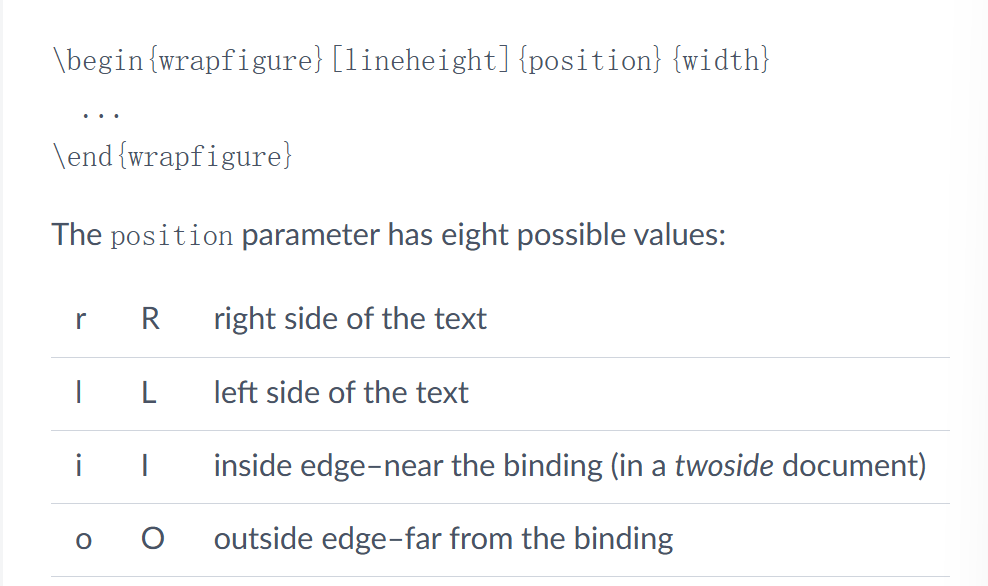
\includegraphics[width=0.5\textwidth]{wrap_figure.png}
\end{wrapfigure}

\end{document}
